\chapter{页表}\label{ch03}

页表是最流行的帮助操作系统为每个进程提供私有地址空间和内存的机制。
页表决定了内存地址的含义和哪些物理内存可以被进程访问。
这允许xv6隔离开不同进程的地址空间并复用同一个物理内存。
页表是一个很流行的设计,因为它们提供了一个间接层,操作系统可以利用这个间接层实现一些技巧。
xv6也使用了一些技巧:把相同的内存(一个trampoline页)映射到多个地址空间中、使用一个未映射的页来保护内核和用户栈。
本章的其余部分解释了RISC-V硬件提供的页表以及xv6如何使用它们。

\section{页表硬件}
提醒一下,RISC-V指令(用户空间和内核空间都是)操作虚拟地址。
机器的RAM,或者说物理内存,是通过物理地址索引的。
RISC-V页表硬件负责连接这两种地址,它把每个虚拟地址映射到物理地址。

xv6在Sv39 RISC-V上运行,意思是只有64位虚拟地址的低39位才会被用到,高25位不使用。
在Sv39配置中,一个RISC-V页表在逻辑上是一个长度为$2^{27}$(134,217,728)的\emph{页表项(page table entries, PTEs)}的数组。
每一个PTE都包含一个44位的物理页号(PPN)和一些标记。
分页硬件在翻译虚拟地址时首先使用39位中的高27位去索引页表,得到一个PTE,然后用其中44位的PPN和39位中的低12位拼接出一个56位的物理地址。
\autoref{f3-1}展示了这个过程,图中简单把页表看做一个PTE的数组(完整的流程见\autoref{f3-2})。
页表允许操作系统以4096($2^{12}$)字节对齐的块为粒度控制虚拟到物理地址的翻译。
这样的一个块被称为一个\emph{页(page)}。

\begin{figure}[htbp]
    \centering
    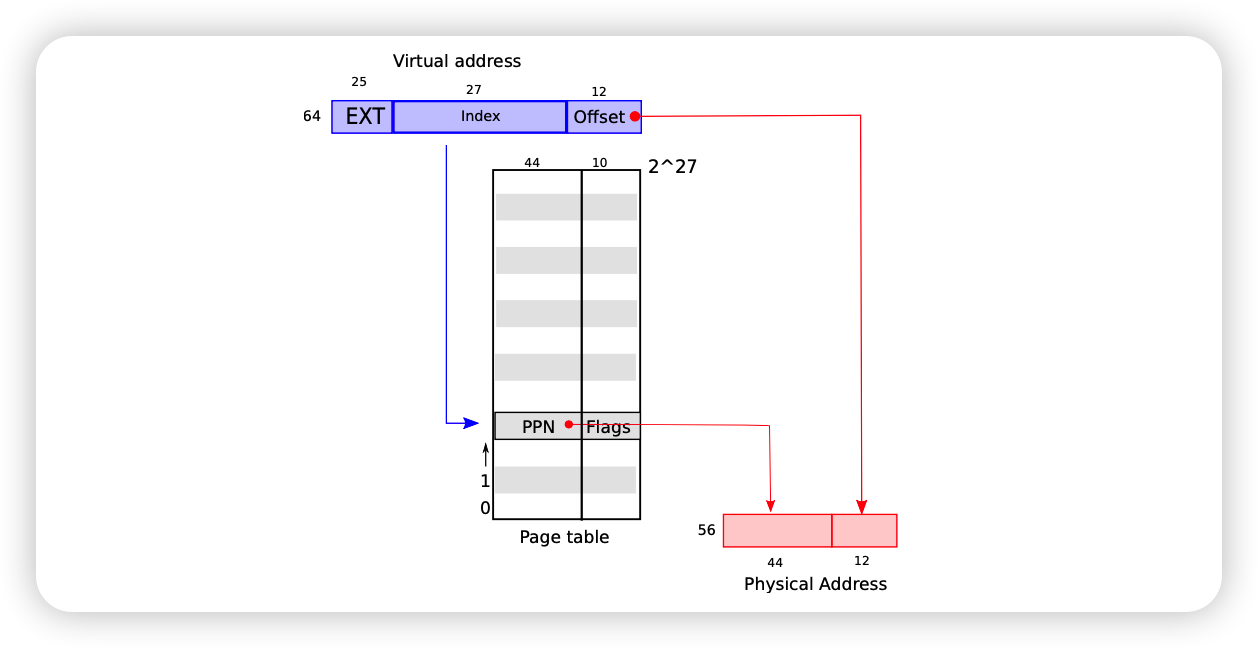
\includegraphics[width=0.8\textwidth]{../imgs/f3-1.png}
    \caption{RISC-V虚拟和物理地址(简化的逻辑页表)}
    \label{f3-1}
\end{figure}

\begin{figure}[htbp]
    \centering
    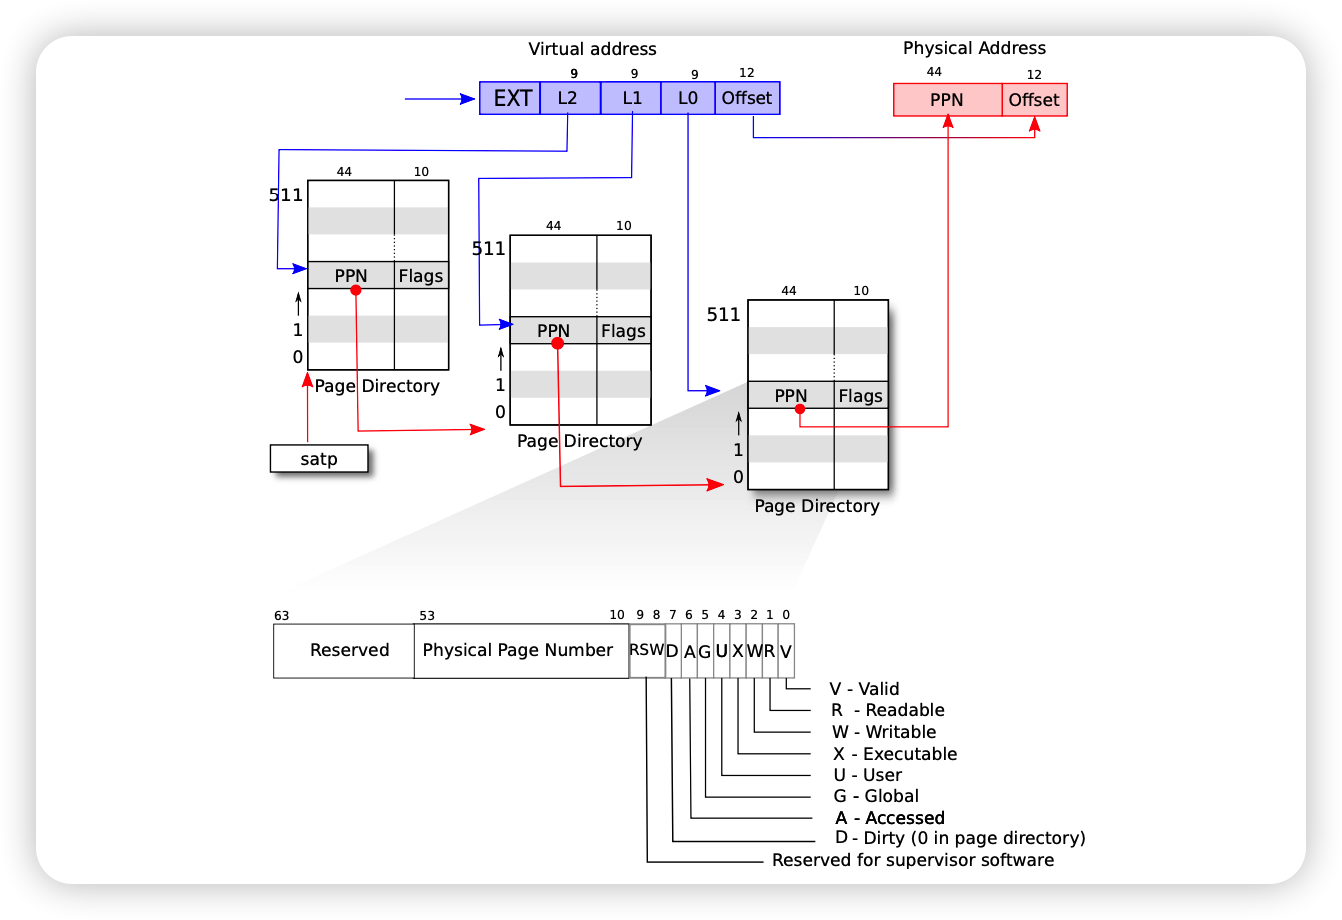
\includegraphics[width=0.8\textwidth]{../imgs/f3-2.png}
    \caption{RISC-V地址翻译细节}
    \label{f3-2}
\end{figure}

在Sv39 RISC-V中,虚拟地址的高25位不用于翻译。
物理地址也还有增长的空间:PTE的格式中还有空间可以让物理页号再增长10位。
RISC-V的设计者根据技术预测选择了这些数字。
$2^{39}$个字节也就是512GB的虚拟地址空间对于运行在RISC-V计算机中的应用来说应该足够了。
$2^{56}$的物理地址空间在不久的未来都足够容纳很多I/O设备和DRAM芯片。
如果还需要更大的空间,RISC-V的设计者还定义了48位虚拟地址的Sv48[3]。

如\autoref{f3-2}所示,一个RISC-V CPU用3步把一个虚拟地址翻译成物理地址。
页表以3级树的形式被存储在物理内存中。
树的根是一个4096字节的页表,它包含512个PTE,每个PTE中都包含了一个下一级页表的物理地址。
每个第二级页表都包含了512个PTE,每个PTE中都包含了树的最后一级。
分页硬件使用27位中的最高9位在根页表中选择一个PTE,用中间9位在第二级页表中选择一个PTE,用低9位去选择最终的PTE。(在Sv48 RISC-V中一个页表有4级,虚拟地址的第39到47位用来在顶级页表索引。)

如果翻译地址所需的三个PTE中的任何一个不存在,分页硬件会抛出一个\emph{页面错误异常(page-fault exception)},让内核来处理这个异常(见\autoref{ch04})。

\autoref{f3-2}中的3级架构与\autoref{f3-1}中的单级设计相比,可以用一种更加内存高效地方式记录PTE。
在通常情况下很大范围内的虚拟地址都没有映射,三级结构可以省略整个页面目录。
例如,如果一个应用只使用了从0开始的很少的页,那么顶级页表的1到511号表项都是无效的,因此kernel不需要为511个中间的页表分配页面。
因此,在这个例子中,3级的设计节省了511个中间的页表和$511 \times 512$个底级页表。

虽然CPU在执行load/store指令时在硬件中运行三级结构,但这种3级架构的一个潜在缺点是在执行load/store指令时CPU必须从内存中加载3个PTE才能把虚拟地址翻译到物理地址。
为了避免从物理内存中加载PTE的开销,RISC-V CPU会把页表项缓存在\emph{翻译查找缓冲区(Translation Look-aside Buffer, TLB)}中。

每个PTE都包含一些标注位,它们告诉分页硬件该虚拟地址允许的操作。
\texttt{PTE\_V}指示PTE是否存在:如果该位未被设置,那么引用对应的页面会导致异常(即不允许)。
\texttt{PTE\_R}控制指令是否可以读取该页。
\texttt{PTE\_W}控制指令是否可以写入该页。
\texttt{PTE\_X}控制指令是否可以把页的内容解释为指令并执行它们。
\texttt{PTE\_U}控制用户模式下的指令是否可以访问该页;如果\texttt{PTE\_U}未被设置,该PTE只能在管理模式下使用。
\autoref{f3-2}展示了所有这些位的含义。
这些标记和所有其他分页硬件相关的结构体定义在\href{https://github.com/mit-pdos/xv6-riscv/blob/risc/kernel/riscv.h}{(kernel/riscv.h)}。

为了让CPU使用页表,内核必须把根页表的物理地址写入\texttt{satp}寄存器。
执行后续的指令时CPU会使用\texttt{satp}指向的页表来翻译所有的地址。
每个CPU都有自己的\texttt{satp},所以不同的CPU可以运行不同的进程,每个进程都有自己的页表所描述的地址空间。

通常内核会把所有物理内存都映射进它的页表里,这样它可以使用load/store指令读取和写入任何物理内存位置。
因为页面目录也在物理内存中,内核可以通过使用标准store指令写入PTE的虚拟地址来编程页面目录中PTE的内容。

解释一下相关的术语。
物理内存是指DRAM的存储单元。
物理内存中的每个字节都有一个地址,称为物理地址。
指令只使用虚拟地址,分页硬件把它翻译成物理地址,然后发送给DRAM硬件以读取或写入存储。
与物理内存和虚拟地址不同,虚拟内存并不是一个物理对象,而是指内核提供的管理物理内存和虚拟地址的抽象和机制的集合。

\section{内核地址空间}
xv6为每个进程维护一个描述用户地址空间的页表,还维护了一个唯一的描述内核地址空间的页表。
内核会设置它的地址空间的布局以让它能访问物理内存和特定虚拟地址处的各种硬件资源。
\autoref{f3-3}展示了怎么把内核虚拟地址映射到物理地址。
文件\href{URL}{(kernel/memlayout.h)}声明了xv6的内核内存布局中的常量。

\begin{figure}[htbp]
    \centering
    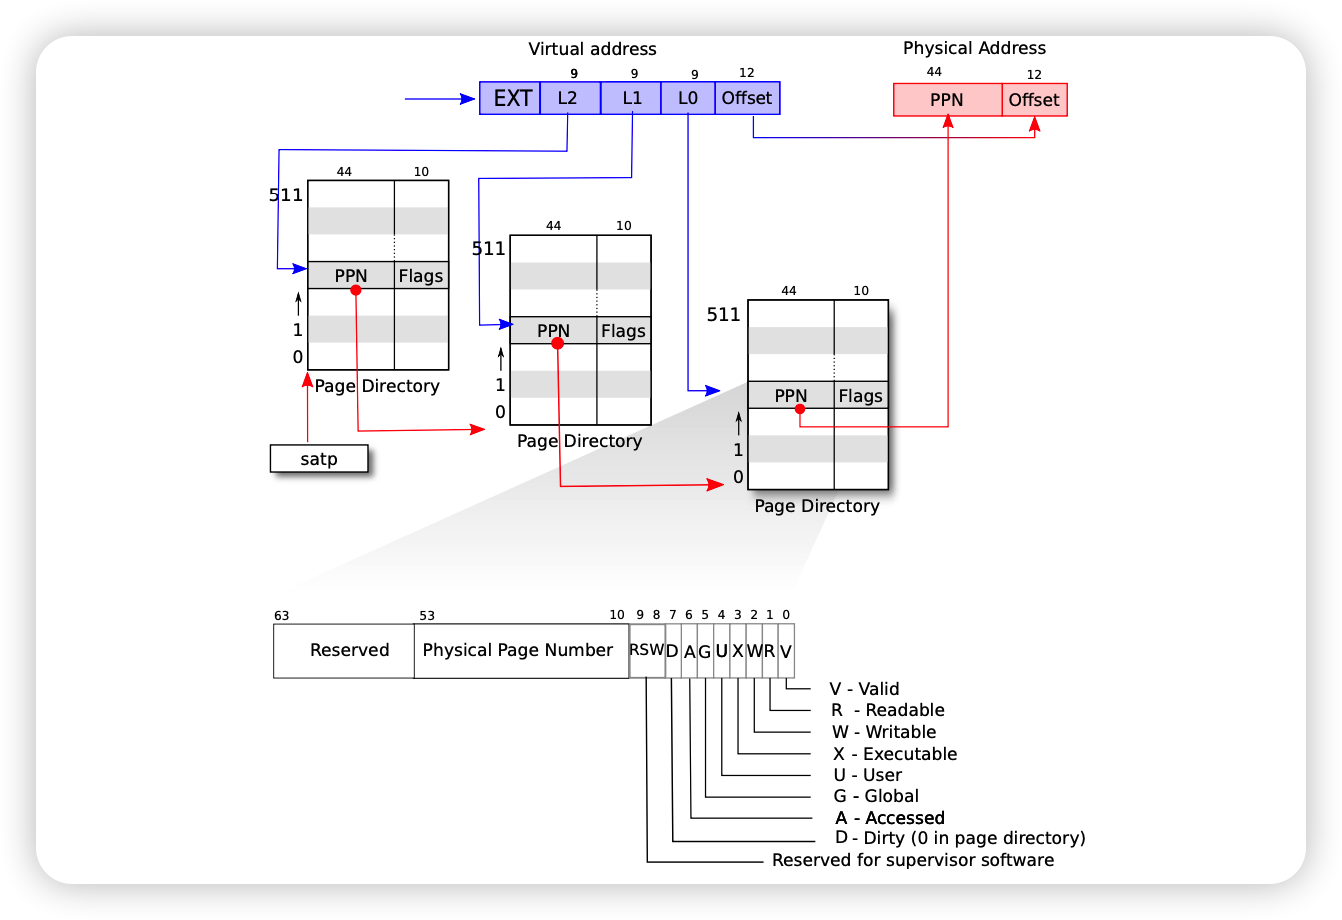
\includegraphics[width=0.8\textwidth]{../imgs/f3-2.png}
    \caption{左侧是xv6的内核地址空间。\texttt{RWX}代表PTE的读、写、执行权限。右侧是xv6期望看到的RISC-V的物理地址空间。}
    \label{f3-3}
\end{figure}

QEMU仿真出的计算机的RAM(物理内存)从物理地址\texttt{0x80000000}开始并至少持续到\texttt{0x88000000},xv6称这个地址为\texttt{PHYSTOP}。
QEMU的仿真也包含I/O设备,例如磁盘。
QEMU以\emph{内存映射(memory-mapped)}控制寄存器的方式把硬件接口暴露给软件,它把设备映射到\texttt{0x80000000}以下的物理内存地址。
内核可以通过读/写特殊的物理地址来和这些设备交互;这样的读/写会和设备硬件而不是RAM进行交互。
\autoref{ch04}会解释xv6怎么和设备交互。

内核使用“直接映射”访问RAM和内存映射设备寄存器,意思是说,把这些资源映射到和物理地址相同的虚拟地址。
例如,内核自身同时位于虚拟地址和物理地址的\texttt{KERNBASE=0x80000000}处。
直接映射简化了读/写物理内存的内核代码。
例如,当\texttt{fork}为子进程分配用户内存时,分配器会返回内存的物理地址,texttt{fork}在把父进程的用户内存拷贝到子进程时可以直接把它用作虚拟地址。

还有一些内核的虚拟地址并不是直接映射:
\begin{itemize}
    \item trampoline页。它被映射到虚拟地址空间的顶部,在用户页表中它也被映射到虚拟地址空间顶部。\autoref{ch04}会讨论trampoline页扮演的角色,但这里我们可以看到一个有趣的页表用例,一个物理页(存储trampoline代码的那个页)在内核的虚拟地址空间中被映射了两次:一次是在虚拟地址空间的顶部,一次是直接映射。
    \item 内核的栈页。每个进程都有自己的内核栈,它被映射到很高的地址处,这样xv6可以在它下面留一个未映射的\emph{保护页(guard page)}。保护页的PTE是无效的(即,\texttt{PTE\_V}位未被设置),这样如果内核溢出了内核栈,它很有可能会触发一个异常,并且内核会崩溃。如果没有守护页,栈溢出时可能会覆盖其他内核内存,导致错误的操作。相对之下崩溃更加可取。
\end{itemize}

尽管内核通过高地址处的映射来使用栈,但使用直接映射的地址也可以访问这些栈。
另一种设计是只使用直接映射,然后使用直接映射地址处的栈。
然而在这种设计中,如果想提供保护页,那么需要取消保护页的虚拟地址映射,否则保护页会映射到物理地址,而这些被取消映射的物理地址将很难再使用起来。

内核以\texttt{PTE\_R}和\texttt{PTE\_X}权限映射trampoline和内核text段的页。
内核将从这些页中读取和执行指令。
内核以权限\texttt{PTE\_R}和\texttt{PTE\_W}映射其他的页面,这样它可以读取和写入那些页面中的内存。
保护页的映射是无效映射。

\section{代码:创建一个地址空间}
xv6中大部分操作地址空间和页表的代码都在\texttt{vm.c}\href{https://github.com/mit-pdos/xv6-riscv/blob/risc/kernel/vm.c#L1}{(kernel/vm.c:1)}中。
其中最主要的数据结构是\texttt{pagetable\_t},它其实是一个指向RISC-V根页表的指针;\texttt{pagetable\_t}要么是内核的页表,要么是进程的页表。
最主要的函数是\texttt{walk}和\texttt{mappages}:\texttt{walk}查找一个虚拟地址对应的PTE,\texttt{mappages}为新的映射添加PTE。
以\texttt{kvm}开头的函数操作内核页表,以\texttt{uvm}开头的函数操作用户页表,其他的函数同时用于两者。
\texttt{copyout}把数据拷贝到用户虚拟地址,\texttt{copyin}相反,地址作为系统调用的参数提供。
它们都在\texttt{vm.c}里,因为它们需要显式地翻译这些地址以找到相应的物理内存。

在启动的早期,\texttt{main}会调用\texttt{kvminit}\href{https://github.com/mit-pdos/xv6-riscv/blob/risc/kernel/vm.c#L54}{(kernel/vm.c:54)},这个函数会使用\texttt{kvmmake}\href{https://github.com/mit-pdos/xv6-riscv/blob/risc/kernel/vm.c#L20}{(kernel/vm.c:20)}创建内核的页表。
这次调用在xv6启用RISC-V的分页功能之前执行,因此其中的地址都直接是物理地址。
\texttt{kvmmake}首先分配一个物理内存页来存储根页表。
然后它调用\texttt{kvmmap}来添加内核翻译地址时需要的映射。
这些映射包括内核的指令和数据、至多到\texttt{PHYSTOP}的物理内存、以及实际上是设备的内存范围。
\texttt{proc\_mapstacks}\href{https://github.com/mit-pdos/xv6-riscv/blob/risc/kernel/proc.c#L33}{(kernel/proc.c:33)}为每个进程分配一个内核栈。
它会调用\texttt{kvmmap}把每个栈映射到\texttt{KSTACK}生成的虚拟地址,以为无效的保护页留出空间。

\texttt{kvmmap}\href{https://github.com/mit-pdos/xv6-riscv/blob/risc/kernel/vm.c#L132}{(kernel/vm.c:132)}会调用\texttt{mappages}\href{https://github.com/mit-pdos/xv6-riscv/blob/risc/kernel/vm.c#L143}{(kernel/vm.c:143)},它把一系列从虚拟地址到物理地址的映射加入到页表中。

\texttt{walk}\href{https://github.com/mit-pdos/xv6-riscv/blob/risc/kernel/vm.c#L86}{(kernel/vm.c:86)}模仿RISC-V的分页硬件查找虚拟地址的PTE的过程(见\autoref{f3-2})。
\texttt{walk}每次用9位逐次查找3级页表。
它使用虚拟地址的每9位去查找下一级页表或者最终目标页的PTE\href{https://github.com/mit-pdos/xv6-riscv/blob/risc/kernel/vm.c#L92}{(kernel/vm.c:92)}。
如果PTE无效,说明请求的页面还没有被分配,如果\texttt{alloc}参数为真,\texttt{walk}会分配一个新的页并把它的物理地址加进PTE里。
它返回树的最底层的PTE的地址\href{https://github.com/mit-pdos/xv6-riscv/blob/risc/kernel/vm.c#L102}{(kernel/vm.c:102)}。

上面的代码依赖于物理内存被直接映射到内核的虚拟地址空间。
例如,\texttt{walk}逐级查询页表时,它从PTE中获取下一级页表的(物理)地址\href{https://github.com/mit-pdos/xv6-riscv/blob/risc/kernel/vm.c#L94}{(kernel/vm.c:94)},然后把它当做一个虚拟地址来获取下一级页表中的PTE\href{https://github.com/mit-pdos/xv6-riscv/blob/risc/kernel/vm.c#L92}{(kernel/vm.c:92)}。

\texttt{main}调用\texttt{kvminithart}\href{https://github.com/mit-pdos/xv6-riscv/blob/risc/kernel/vm.c#L62}{(kernel/vm.c:62)}来安装页表。
它把根页表的物理地址存入\texttt{satp}寄存器。
之后CPU就会使用内核的页表翻译所有的地址。
因为内核使用了直接映射,现在下一条指令的虚拟地址将会映射到正确的物理内存地址。

每一个RISC-V CPU都会页表项缓存到\emph{翻译查找缓冲区(Translation Look-aside Buffer, TLB)}中,所以当xv6修改一个页表时,它必须告诉CPU把相应的缓存的TLB条目无效化。
如果不这么做,之后TLB可能会使用旧的映射,旧的映射可能指向一个现在已经被分配给别的进程的物理页,这样一个进程就可能扰乱其他进程的内存。
RISC-V有一条指令\texttt{sfence.vma}用来清空当前CPU的TLB。
xv6在\texttt{kvminithart}中修改\texttt{satp}寄存器之后执行了\texttt{sfence.vma},trampoline代码中在返回用户空间之前会先切换到用户的页表,之后也要执行\texttt{sfence.vma}\href{https://github.com/mit-pdos/xv6-riscv/blob/risc/kernel/trampoline.S#L89}{(kernel/trampoline.S:89)}。

在修改\texttt{satp}之前执行\texttt{sfence.vma}也是必要的,这是为了等待所有load/store指令的完成。
这可以保证之前对页表的更新已经完成,也确保之前的load和store都是用的旧的页表,而不是新的。

为了避免清空整个TLB,RISC-V CPU可以支持地址空间标识符(ASID)[3]。
这样内核可以只情况特定地址空间的TLB条目。
xv6并没有用到这个feature。

\section{物理内存分配}

